\documentclass[10pt,a5paper]{article}
\usepackage[utf8]{inputenc}
\usepackage[portuguese]{babel}
\usepackage[backend=bibtex,
style=numeric,
sorting=none
]{biblatex}
\addbibresource{bibfile.bib}
\usepackage{amsmath}
\usepackage{amsfonts}
\usepackage{amssymb}
\usepackage{graphicx}
\usepackage{hyperref}
\usepackage{indentfirst} %Force identation after section
\usepackage{tabularx}
\usepackage{ragged2e}  % for "\RaggedRight" macro
\usepackage{longtable}
\usepackage{rotating}
\usepackage{geometry}
\usepackage{etoolbox}
\usepackage{subcaption}

%%%%%%%%%%%%%%%%%%%%%%%%%%%%%%%%%%%%%%% DOCUMENT SETUP %%%%%%%%%%%%%%%%%%%%%%%%%%%%%%%%%%%%%%%%%%%%%%%%%%%%

% Allow more then 3 section levels
\makeatletter
\renewcommand\paragraph{\@startsection{paragraph}{4}{\z@}%
	{-2.5ex\@plus -1ex \@minus -.25ex}%
	{1.25ex \@plus .25ex}%
	{\normalfont\normalsize\bfseries}}
\makeatother
\setcounter{secnumdepth}{4} % how many sectioning levels to assign numbers to
%\setcounter{tocdepth}{4}    % how many sectioning levels to show in ToC

% Allow landscape
\makeatletter
\def\ifGm@preamble#1{\@firstofone}
\appto\restoregeometry{%
	\pdfpagewidth=\paperwidth
	\pdfpageheight=\paperheight}
\apptocmd\newgeometry{%
	\pdfpagewidth=\paperwidth
	\pdfpageheight=\paperheight}{}{}
\makeatother

%%%%%%%%%%%%%%%%%%%%%%%%%%%%%%%%%%%%%%%%%%%%%%%%%%%%%%%%%%%%%%%%%%%%%%%%%%%%%%%%%%%%%%%%%%%%%%%%%%%%%%%%%%%
\title{IoT - Waste Management System}

\begin{document}

\begin{titlepage}
	
	\newcommand{\HRule}{\rule{\linewidth}{0.5mm}} % Defines a new command for the horizontal lines, change thickness here
	
	\center % Center everything on the page
	
	%--------------------------------------------------------------------------------------
	%	CABEÇALHO
	%---------------------------------------------------------------------------------------
	
	\begin{figure}
		
\includegraphics[width=0.5\textwidth]{Images/app_logo}
	\end{figure}
	
	%----------------------------------------------------------------------------------------
	%	TITULO
	%----------------------------------------------------------------------------------------
	
	\HRule \\[0.2cm]
	{ \huge \bfseries Waste Management Mobile Application}\\
%	{ \big \bfseries Otimização das rotas de recolha}\\[0.3cm]
	\vspace*{10px}
	{\Large Manual de Utilização}
	\HRule \\[0.8cm]
	

	%----------------------------------------------------------------------------------------
	\vfill % Fill the rest of the page with whitespace
	
\end{titlepage}


\cleardoublepage

\tableofcontents

\pagenumbering{arabic}

\cleardoublepage

\section{Dicionário de ícones}
Na aplicação móvel existe um conjunto de ícones que são reaproveitados nos vários ecrãs que esta disponibiliza, sendo estes apresentados na Tabela \ref{tbl:table_of_figures}, juntamento com o seu significado.

\newcolumntype{C}{>{\centering\arraybackslash}m{6em}}

\begin{table}[!h]
	\centering
	\begin{tabular}{Cc}
		\textbf{Figura} & \textbf{Descrição} \\ \hline
		\vspace*{3px}
		
\includegraphics[width=0.1\textwidth]{Images/icons/temperature_icon} & Valor da temperatura interior do contentor\\ \hline
		
\includegraphics[width=0.1\textwidth]{Images/icons/occupancy_icon} & Taxa de ocupação do contentor\\ \hline		
		
\includegraphics[width=0.1\textwidth]{Images/icons/battery_icon} & Valor da bateria do sistema embebido instalado no contentor\\ \hline
		
\includegraphics[width=0.1\textwidth]{Images/icons/location} & Coordenadas relativas à localização de um elemento da rede\\ \hline
	\end{tabular}
	\caption{Dicionário de ícones}
	\label{tbl:table_of_figures}
\end{table}

\section{Manual de Utilização}
Nesta secção é descrito o modo de utilização da aplicação.

\newpage
\subsection{\textit{Login}} 

\begin{figure}[!h]
	\centering
	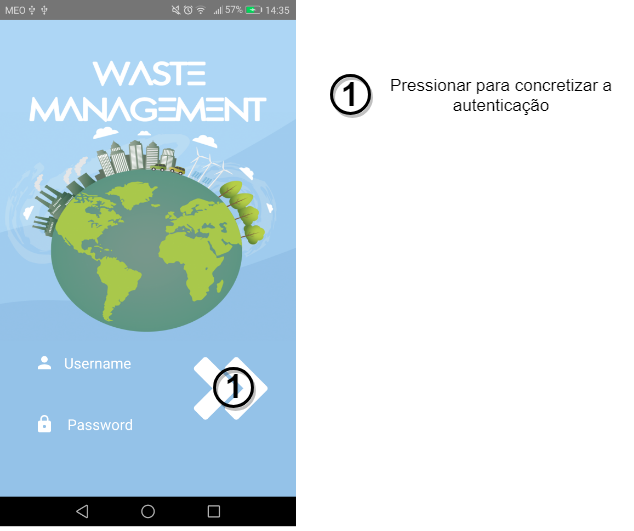
\includegraphics[width=1.1\textwidth]{Images/screens/login_screen}
	\caption{Ecrã de \textit{Login}}
	\label{fig:login_screen}
\end{figure}

\newpage
\subsection{Gestão ou Administração} 

\begin{figure}[!h]
	\centering
	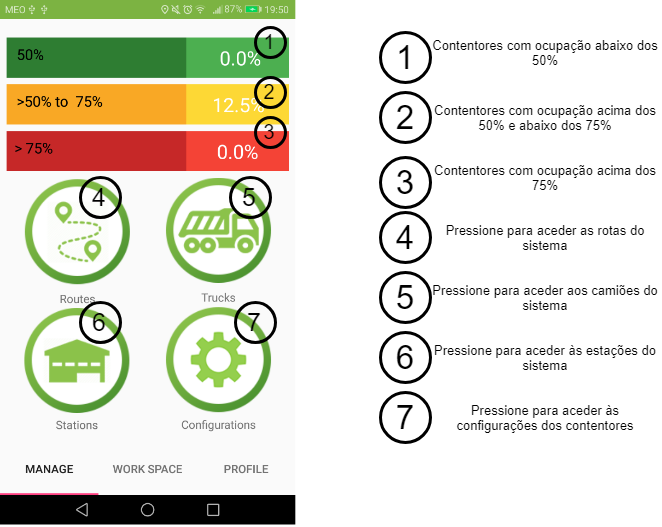
\includegraphics[width=1.1\textwidth]{Images/screens/manage_screen_frag}
	\caption{Ecrã de Gestão}
	\label{fig:manage_screen_frag}
\end{figure}

\newpage
\subsection{Rotas} 

\begin{figure}[!h]
	\centering
	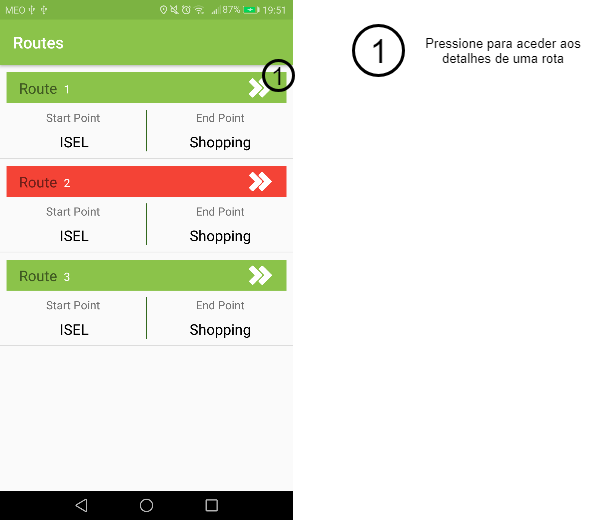
\includegraphics[width=1.1\textwidth]{Images/screens/routes_screenxml}
	\caption{Ecrã com todas as rotas}
	\label{fig:routes_screen}
\end{figure}

\newpage
\subsection{Camiões} 

\begin{figure}[!h]
	\centering
	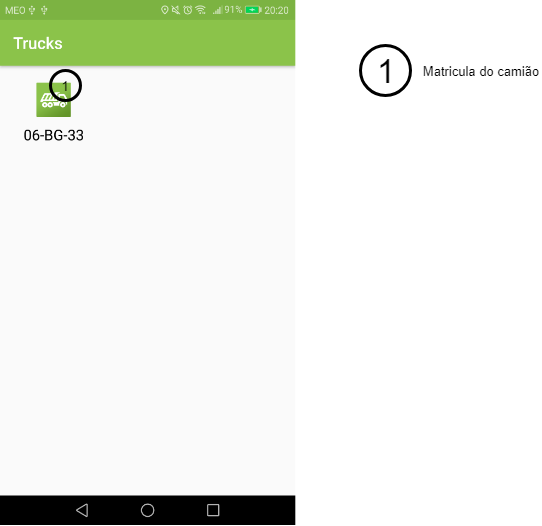
\includegraphics[width=1.1\textwidth]{Images/screens/trucks_screen}
	\caption{Ecrã com todos os camiões}
	\label{fig:trucks_screen}
\end{figure}

\newpage
\subsection{Estações} 

\begin{figure}[!h]
	\centering
	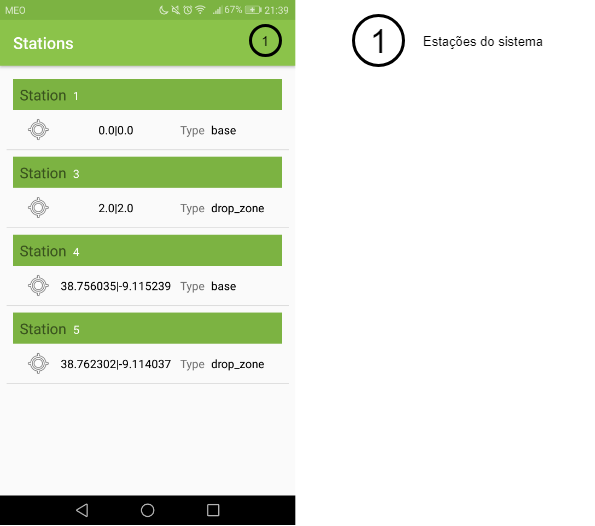
\includegraphics[width=1.1\textwidth]{Images/screens/stations_screen}
	\caption{Ecrã com todas as estações}
	\label{fig:stations_screen}
\end{figure}

\newpage
\subsection{Configurações} 

\begin{figure}[!h]
	\centering
	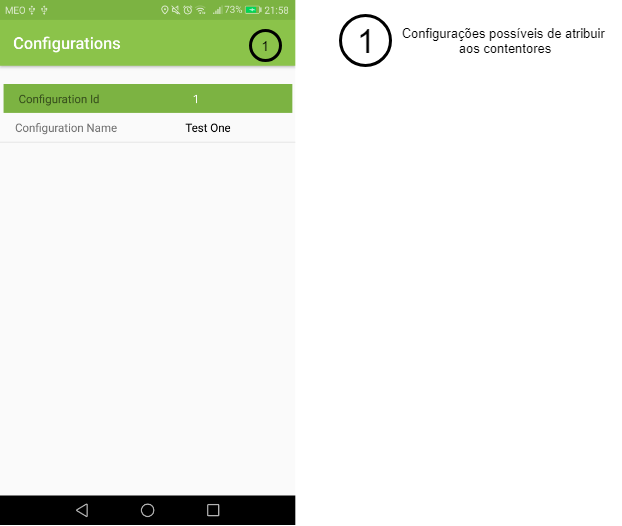
\includegraphics[width=1.1\textwidth]{Images/screens/configurations_screen}
	\caption{Ecrã com todas as configurações}
	\label{fig:configurations_screen}
\end{figure}

\newpage
\subsection{Detalhes da rota} 

\begin{figure}[!h]
	\centering
	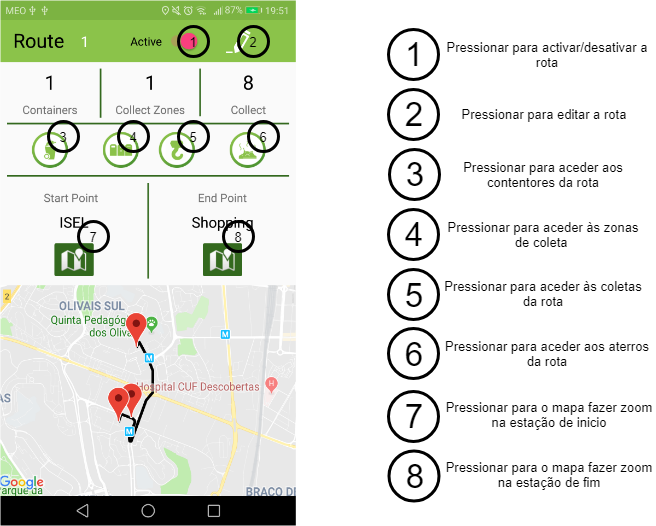
\includegraphics[width=1.1\textwidth]{Images/screens/route_screen}
	\caption{Ecrã com detalhes de uma rota}
	\label{fig:route_screen}
\end{figure}

\newpage
\subsection{Contentores de uma rota} 

\begin{figure}[!h]
	\centering
	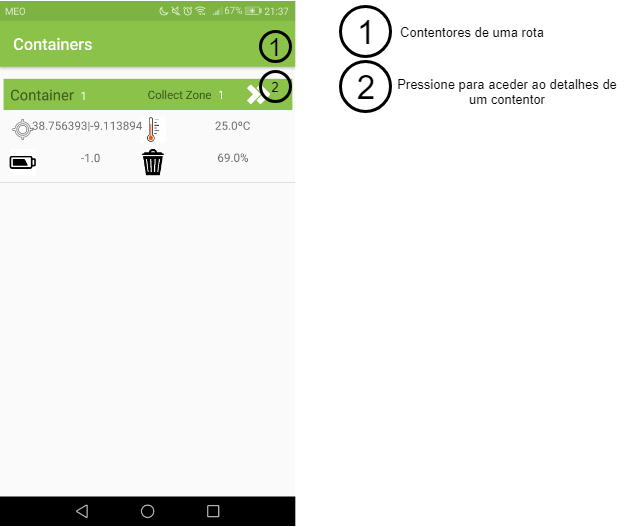
\includegraphics[width=1.1\textwidth]{Images/screens/route_containers_screen}
	\caption{Ecrã com os contentores de uma rota}
	\label{fig:route_containers_screen}
\end{figure}

\newpage
\subsection{Zonas de coleta de uma rota} 

\begin{figure}[!h]
	\centering
	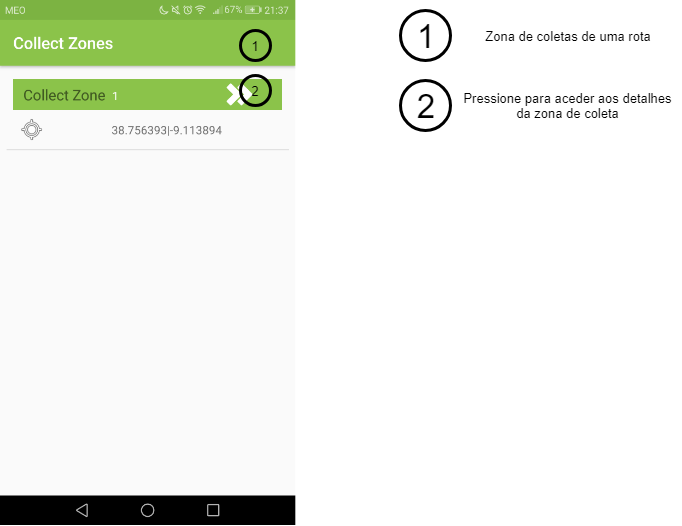
\includegraphics[width=1.1\textwidth]{Images/screens/collect_zones_screen}
	\caption{Ecrã com as zonas de coleta de uma rota}
	\label{fig:collect_zones_screen}
\end{figure}

\newpage
\subsection{Coletas de uma rota} 

\begin{figure}[!h]
	\centering
	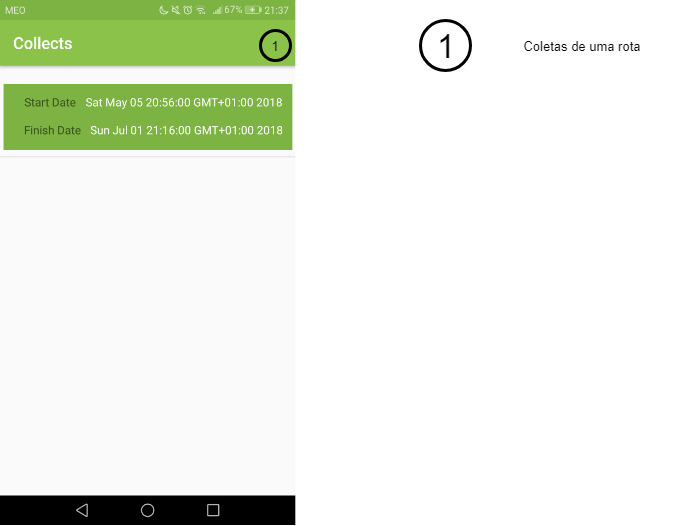
\includegraphics[width=1.1\textwidth]{Images/screens/route_collects}
	\caption{Ecrã com as coletas de uma rota}
	\label{fig:route_collects}
\end{figure}

\newpage
\subsection{Aterros de uma rota} 

\begin{figure}[!h]
	\centering
	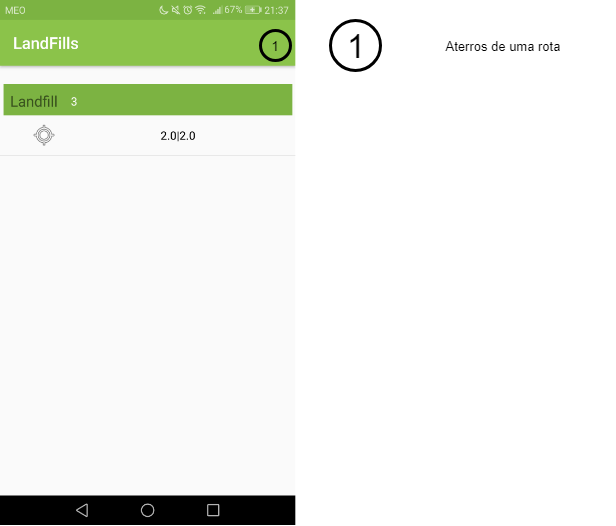
\includegraphics[width=1.1\textwidth]{Images/screens/route_landfills}
	\caption{Ecrã com os aterros de uma rota}
	\label{fig:route_landfills}
\end{figure}

\newpage
\subsection{Detalhes de uma zona de coleta} 
\begin{figure}[!h]
	\centering
	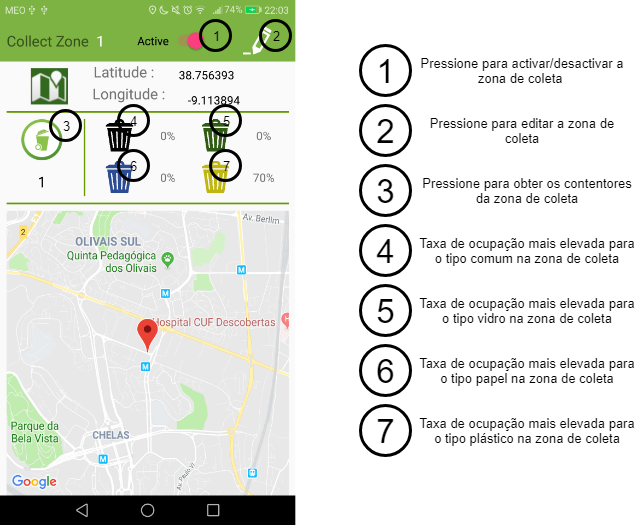
\includegraphics[width=1.1\textwidth]{Images/screens/collect_zone_screen}
	\caption{Ecrã com os detalhes de uma zona de coleta}
	\label{fig:collect_zone_screen}
\end{figure}

\newpage
\subsection{Contentores de uma zona de coleta} 

\begin{figure}[!h]
	\centering
	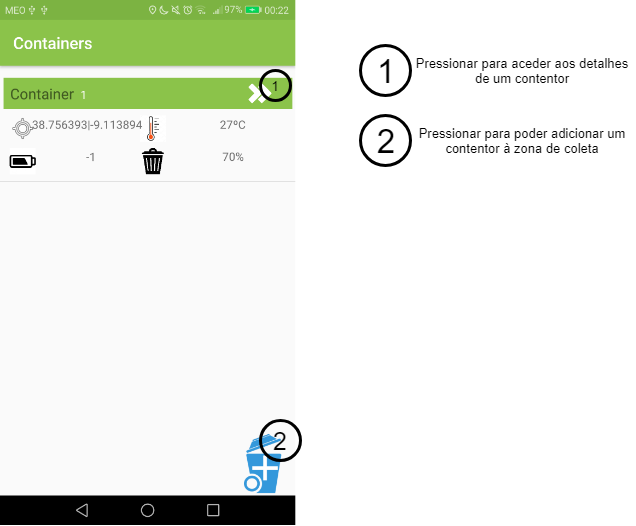
\includegraphics[width=1.1\textwidth]{Images/screens/collect_zones_containers_screen}
	\caption{Ecrã com os contentores de uma zona de coleta}
	\label{fig:collect_zones_containers_screen}
\end{figure}

\newpage
\subsection{Detalhes de um Contentor} 
\begin{figure}[!h]
	\centering
	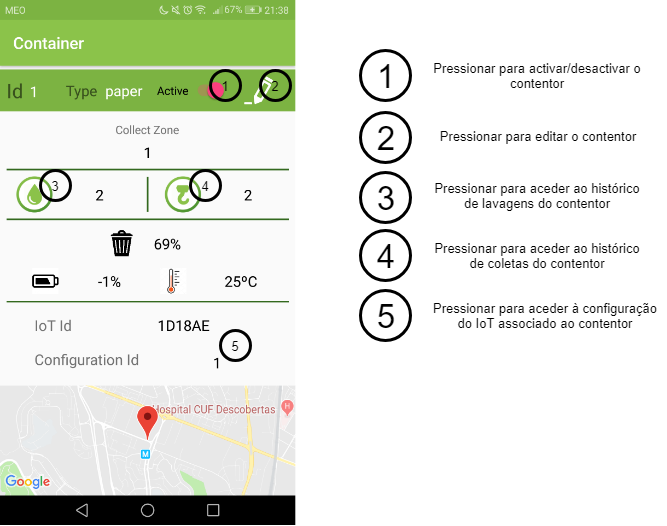
\includegraphics[width=1.1\textwidth]{Images/screens/container_screen}
	\caption{Ecrã com os detalhes de um contentor}
	\label{fig:container_screen}
\end{figure}

\newpage
\subsection{Histórico de coletas de um Contentor} 

\begin{figure}[!h]
	\centering
	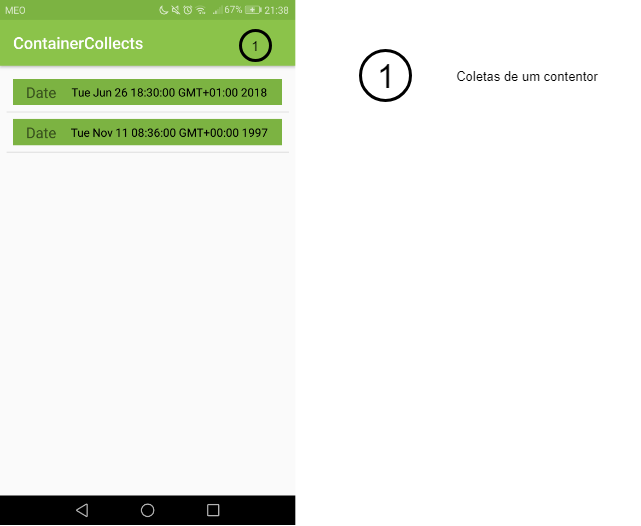
\includegraphics[width=1.1\textwidth]{Images/screens/container_collects}
	\caption{Ecrã com o histórico de coletas de um contentor}
	\label{fig:container_collects}
\end{figure}

\newpage
\subsection{Histórico de lavagens de um Contentor} 

\begin{figure}[!h]
	\centering
	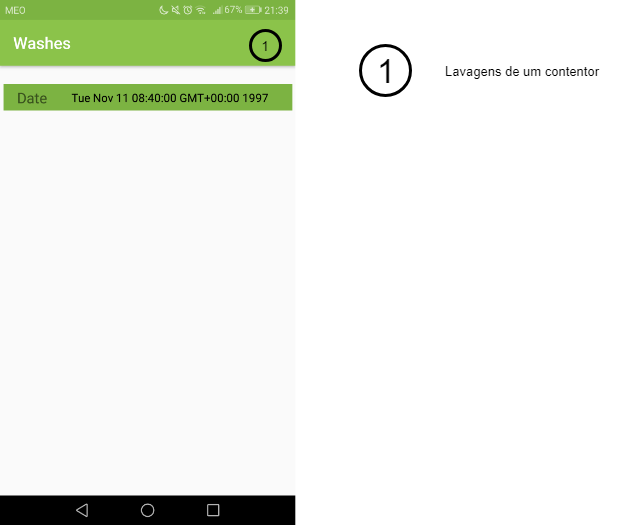
\includegraphics[width=1.1\textwidth]{Images/screens/container_washes}
	\caption{Ecrã com o histórico de lavagens de um contentor}
	\label{fig:container_washes}
\end{figure}

\newpage
\subsection{Configurações de um Contentor} 

\begin{figure}[!h]
	\centering
	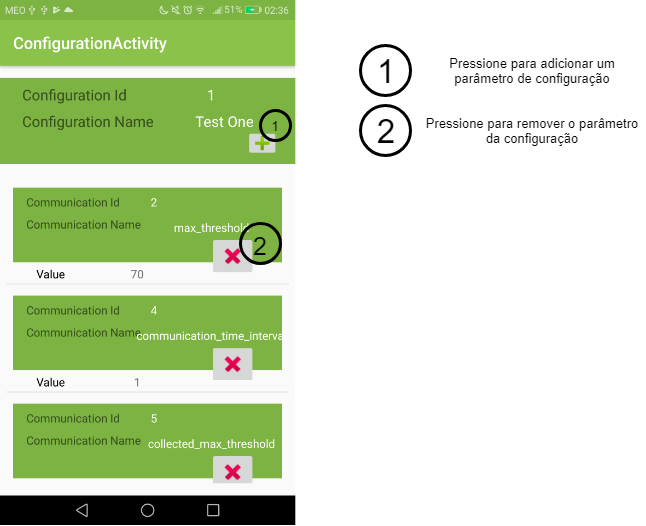
\includegraphics[width=1.1\textwidth]{Images/screens/container_configuration}
	\caption{Ecrã com as configurações de um contentor}
	\label{fig:container_configuration}
\end{figure}

\newpage
\subsection{Coletor} 

\begin{figure}[!h]
	\centering
	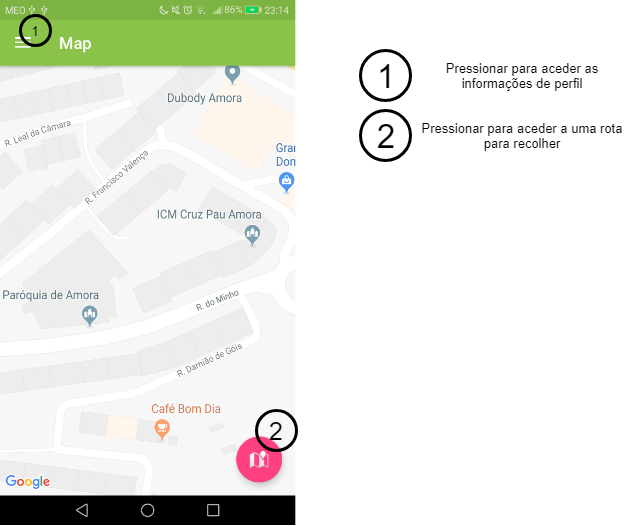
\includegraphics[width=1.1\textwidth]{Images/screens/collector}
	\caption{Ecrã do coletor}
	\label{fig:collector}
\end{figure}

\newpage
\subsection{Coletor terminar a coleta} 

\begin{figure}[!h]
	\centering
	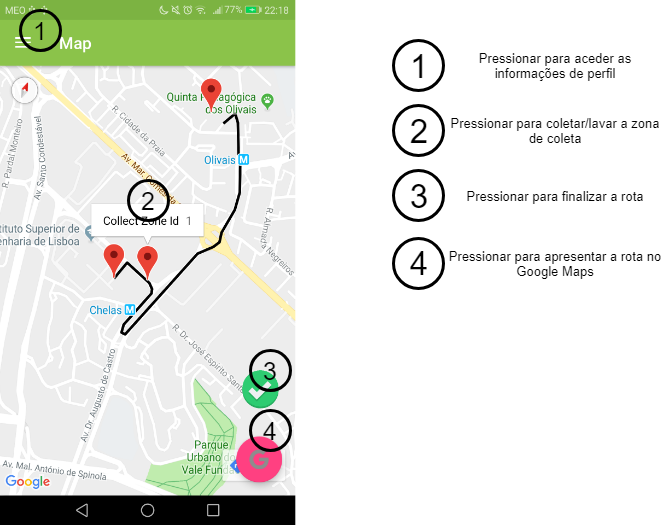
\includegraphics[width=1.1\textwidth]{Images/screens/collector_finish}
	\caption{Ecrã para terminar a coleta}
	\label{fig:collector_finish}
\end{figure}

\end{document}